\chapter{Evaluation}\label{Eval}
This chapter is the evaluation of the script based on the Google Lighthouse audit. This chapter will highlight some elements of the audit. The full audit can be seen in appendix \ref{Audit}. The given score in the relevant categories can be seen in figure x. There was a bug in the measurement of the performance score, resulting in a score of 0. The actual score have been manually calculated in the end of section \ref{EvalPerform}. 

\begin{figure} [H]
	\centering
	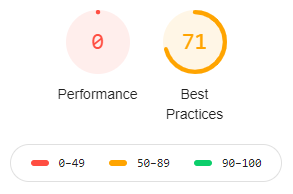
\includegraphics[width=.4\textwidth]{Pictures/LighthouseGrade}
	\caption{The score for performance and best pratices from Google Lighthouse}
	\label{LighthouseGrade}
\end{figure}

\subsection{Performance}\label{EvalPerform}
As shown the performance scored zero out of one hundred. The performance in each of the metrics can be seen in figure \ref{PerformanceAuditValues}.

\begin{figure} [H]
	\centering
	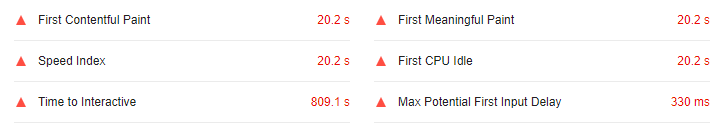
\includegraphics[width=.8\textwidth]{Pictures/PerformanceAuditValues}
	\caption{The result of the performance audit}
	\label{PerformanceAuditValues}
\end{figure}
\fxnote{Remove potential first input delay from figure?}

It does seem like some bug in the tool must have occurred because all of the values are too high. This can be confirmed by comparing with the measurements from the developer tool’s performance tool. These show that the page is fully loaded in 4.6 second, which does not fit with Lighthouse’s 20.2 seconds for First Contentful and First Meaningful Paint. Another sign that something is amiss is the 13.5 minutes before the Time to Interactive, which the tool determined within 10 seconds of analyzing the site. 

Even if the automatic calculation of the performance metrics failed the metrics are still relevant for the evaluation. Using the data from the performance tool these values can be manually estimated. 

\begin{figure} [H]
	\centering
	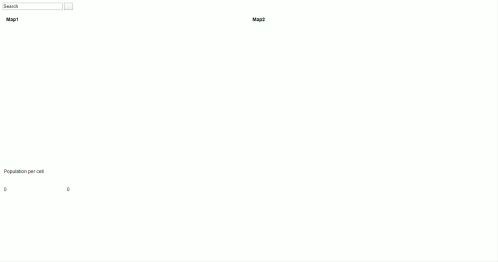
\includegraphics[width=.8\textwidth]{Pictures/ScreenshotLoading1}
	\caption{After 0.3 seconds the search bar and legend appears.}
	\label{ScreenshotLoading1}
\end{figure}

Figure x, x and x are all screenshots of the website taken by the performance tool, while the page was loading. Figure x is taken 0.3 seconds after the page started loading. This time is both the First Meaningful Paint and First CPU Idle since the user can interact with the searchbar.

\begin{figure} [H]
	\centering
	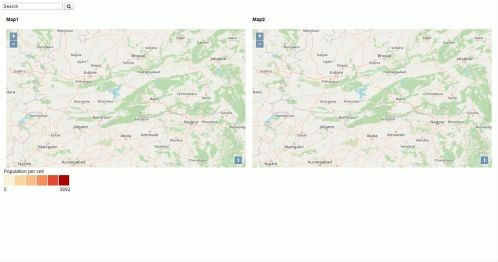
\includegraphics[width=.8\textwidth]{Pictures/ScreenshotLoading2}
	\caption{After 1 second the map appears without the raster layer}
	\label{ScreenshotLoading2}
\end{figure}

After 1 second the maps appear on the website as shown in figure x. The user is able pan and zoom in the map, so this is the Time to Interactive. 

\begin{figure} [H]
	\centering
	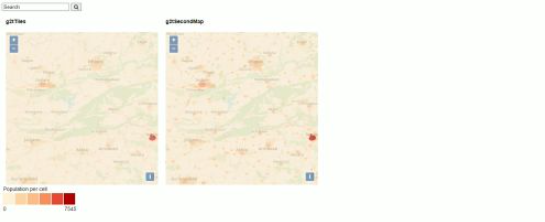
\includegraphics[width=.8\textwidth]{Pictures/ScreenshotLoading3}
	\caption{After 4.6 seconds the map is fully loaded}
	\label{ScreenshotLoading3}
\end{figure}

The last screenshot at figure x shows the map fully loaded after 4.6 seconds. With the tiff tiles being loaded and visualized this is the time for the First Meaningful Paint. This can be used as a conservative estimate for the Speed Index. This would be the value for the Speed Index if everything got visualized at this time and nothing had been visualized on the website prior.

The real Speed Index would be lower, since the legend, map titles and search bar have been visualized at an earlier stage. 

These metrics can then manually be calculated into a score using the Lighthouse Scoring Calculator as shown in figure x. The calculator in unable to take inputs below 1 second. Based on the given value the performance should have scored 88.
https://googlechrome.github.io/lighthouse/scorecalc/

\begin{figure} [H]
	\centering
	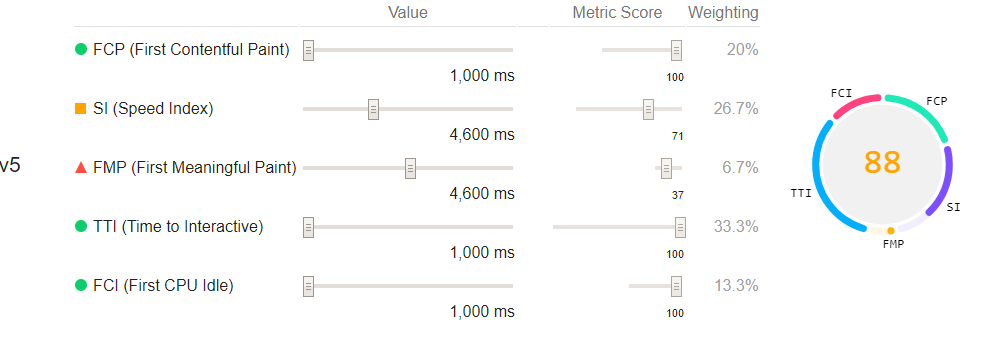
\includegraphics[width=.8\textwidth]{Pictures/ScoringManual}
	\caption{The website for manually calculating the scores, which Lighthouse grants}
	\label{ScoringManual}
\end{figure}

\fxnote{Update to new scoring and time numbers }

\subsection{Opportunities}
In addition to providing the metrics for the performance Lighthouse also comes with suggestion to how the loading time can be reduced. The points listed here will be elaborated upon further in the discussion.

\textbf{Eliminate render-blocking resources}\\
The opportunity for the largest estimated time saving is to eliminate render-blocking resources. These are the URLs, which must be loaded before the first paint can be applied to the page. \citep{RenderBlocking}

Table x shows the different libraries, which have to be loaded before the site is rendered. It can be seen that Openlayers is 82 \% of the loaded data.
\fxnote{Have I written about Jquery??}

\fxnote{Have I explained the difference between HTTP 1 and 2?}

\begin{table}[htbp]
	\centering
	\begin{tabular}{l}
		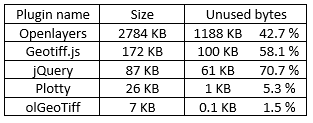
\includegraphics[width=0.6\textwidth]{Pictures/tabPluginSize}
	\end{tabular}
	\caption{Size of loaded modules and the much they are used}
	\label{tabPluginSize}
\end{table}

When analysed further with the Coverage tool it can be seen that a large part of the Openlayers library is not being used as show in table \ref{tabPluginSize}.  
\fxnote{TODO: Make a table from the information in the figure below – tabtext – resourse use of the 3 larges libraries}

\fxnote{Write about Coverage earlier – maybe in evaluation tools}

\textbf{Minification and compressing}\\
Files sizes and script parsing time can be reduced by minifying and compressing the files. 

A minified file is a file, where all the unnecessary parts have been cut away. Whitespaces and unused code are removed leaving a smaller file, which still functions perfectly. 

Compression is using an algorithm to modify the data, so that it takes up less space.
\citep{MinifyJS}

\textbf{Avoid enormous network payloads}\\
Long loading times are highly correlated with the amount of loaded data.  
\citep{LoadingTooMuch}

Loading the raster tiles for the map does require loading multiple files with a large bit depth, which requires a lengthy loading time. 

\textbf{Does not use HTTP/2 for all of its resources}\\
This suggested improvement appears if some of the page’s resources are being served with a version of HTTP/1. According to Google Audit all loaded resources are being delivered using HTTP 1.1.

\fxnote{Write about HTTP/2 earlier?}

\citep{HTTP2}

\textbf{Uses deprecated APIs}\\
When loading the metadata about the tiles a synchronous XMLRequest is used. This is a deprecated API, which will be removed from Chrome in a feature edition. 
\citep{OldApis}
\fxnote{borgerinddragelses værktøj}
\section{Postload performance}

In addition to the measurements of the performance for loading the site the performance after loading was also measured. In table \ref{tabPostloadPerformance} is measurements of performance of using the tool. It can be seen that loading and coloring a new layer takes 3.89 seconds, whereas coloring a layer, which already have been loaded takes on average 0.56 seconds. 
\fxnote{In section x is a further explaination for the larger variance in the recoloring measurements}

\begin{figure} [H]
	\centering
	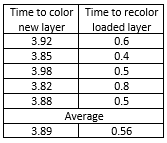
\includegraphics[width=.4\textwidth]{Pictures/tabPostloadPerformance}
	\caption{Seconds to load a new layer and color it and to recolor a loaded layer}
	\label{tabPostloadPerformance}
\end{figure}